\documentclass[11pt]{article}
\usepackage{colacl}
\usepackage{graphicx}
\sloppy



\title{Knowledge Technology Assignment1 Semester1}
\author{Xiaodong Han 822581}



\begin{document}
\maketitle

\section{Introduction}
In this project, the assignment is to represent the Latin word by giving a representation word in Persian script. The problem is that there is no exact match in this process. Thus, the mechanism for representing the Latin word is to treat (uppercase) Persian name as a “misspelled” versions of the Latin names; using approximate match methods to return the best-scored name(s) to users. This report will discuss three different approximate methods, Global Edit Distance (GED), N-Gram Distance, and Local Edit Distance (LED), and evaluate these methods by using some metric like precision and recall.



\section{Data-sets}
All resource data-sets (names.txt, train.txt) used in this report are given by \newcite{Karimi2006English}. File names.txt contains a bunch of Latin names, which will probably be the dictionary; file train.txt contains a bunch of Persian names with their (correct) Latin equivalent.


\section{Global Edit Distance}
In this section, calculating the different GED between each (uppercase) Persian name in train.txt and all (lowercase) Latin names in names.txt. The best-scoring Latin name(s) from names.txt is/are the prediction(s), which can be compared with the true (lowercase) Latin name in train.txt to verify whether it is correct. In particular, using different parameter will return different result.

\subsection{Using Basic Parameter}
Using parameter [m, i, d, r] = [+1, -1, -1, -1], which is a basic parameter.The performance is as follow: (see Table~\ref{table1}).

\begin{table}[h]
 \begin{center}
\begin{tabular}{|l|l|}

      \hline
      Metric & Proportion\\
      \hline\hline
      Precision & 6207/43056=14.416\%\\
      Recall & 6207/13437=46.193\%\\
      \hline

\end{tabular}
\caption{Performance of Global Edit Distance}\label{table1}
\end{center}
\end{table}

Table1 shows the performance of using basic parameter, but the precision in this table is not ideal. This is because basic parameter only considers the numbers of edit operations without taking into account the fact that the same operation for different character pairs has different weights and even different operations for same character pair have different weight. For example, for same character pair ‘K’ and ‘c’, replacement may have higher weight than delectation, since ‘K’ and ‘c’ have similar pronunciation. Thus, it is not accurate to give all characters a same operation weight.

 

\subsection{Modifying 'r' Parameter}
Based on the observation of train.txt, I find that, in the process of transliteration between Persian name and Latin name, there are a lot of replacements between different characters which have the same pronunciation in English. I assume that the pronunciation of Persian name and Latin name follows English pronunciation rules, so that I can use Soundex code rule to divide all characters into six groups and ignore character ` which appears very few times. Thus, when calculating the distance, if two characters are involved in the same group, then the replacement counts 0, whereas replacement counts -1. Based on this rule, I modify a new parameter, which is [m, i, d, r] = [+1, -1, -1, (-1, 0)]. The performance of using new parameter is as follow: (see Table~\ref{table2}).

\begin{table}[h]
 \begin{center}
\begin{tabular}{|l|l|}

      \hline
      Metric & Proportion\\
      \hline\hline
      Precision & 7342/44531=16.487\%\\
      Recall & 7342/13437=54.640\%\\
      \hline

\end{tabular}
\caption{Performance of Global Edit Distance}\label{table2}
\end{center}
\end{table}

This performance shows that both precision and recall are increased, which means the number of incorrect names returned is decreased and the number of correct names is increased. There are two main discoveries based on this improvement. First of all, in the process of transliteration of Persian name and Latin name, characters having the similar pronunciation have the large proportion of being replaced. Secondly, Persian and Latin may have the same pronunciation with English. Taking Persian name “ABDVN” as an example, the exact Latin name is “ebdon”. Using GED with basic parameter, the best-scored match is “labdon”, in this case, the accuracy of matching this word is 0\%. While using GED with new parameter, the best-scored matches are “ebdon” and “labdon”, and the accuracy is 50\%. 

\setlength{\parskip}{0.5\baselineskip}

In order to further improve efficiency, I calculate the frequency of characters appearing in Latin name, see Figure~\ref{fig}.
\begin{figure}[htbp] 
\centering
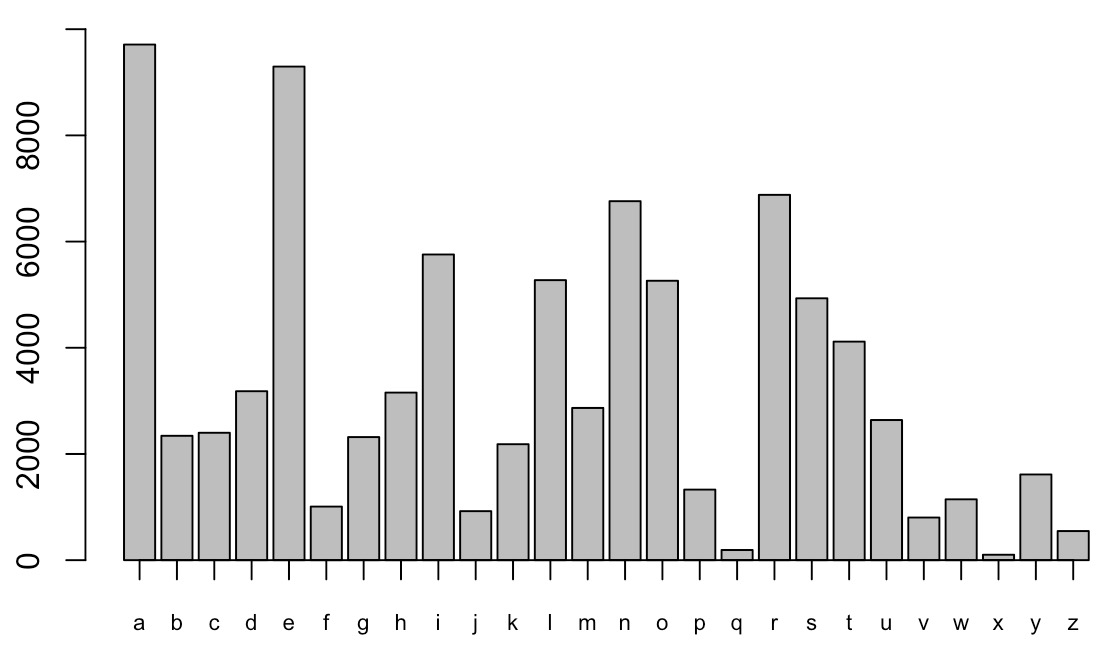
\includegraphics[width=3.2in]{frequencyinLatin} 
\caption{Frequency of characters appearing in Latin names}\label{fig} 
\end{figure} 
\par
As it shows in the ~\ref{fig}, based on the Soundex code rules, the average frequency of characters in group (a, e, h, i, o, u, w, y) appearing in Latin name is larger than other groups. That means characters in group (a, e, h, i, o, u, w, y) have higher possibility appearing in Latin name. Thus, when calculating the distance, if two characters are involved in group (a, e, h, i, o, u, w, y), then the replacement counts 1, while if two characters are involved in the same group but not group (a, e, h, i, o, u, w, y), then the replacement counts 0, and in other cases, the replacement counts -1. The new parameter is [m, i, d, r] = [+2, -1, -1, (-1, 0, 1)], the performance of this parameter is as follow: (see Table~\ref{table3}).

\begin{table}[h]
 \begin{center}
\begin{tabular}{|l|l|}

      \hline
      Metric & Proportion\\
      \hline\hline
      Precision & 7439/31044=23.963\%\\
      Recall & 7439/13437=55.362\%\\
      \hline

\end{tabular}
\caption{Performance of Global Edit Distance}\label{table3}
\end{center}
\end{table}

Different with second modified parameter, this one decreases the number of incorrect names, which has increased the precision of this system. For example, the exact Latin name which matching the Persian name "AGLSTVN" is "eaglestone"; for GED with basic parameter, it only care about operation times; for GED with second modified parameter, it does not distinguish the different weightes towards different Soundex-code-group; so that only GED with third modified parameter can predict this kind of words.


% \setlength{\parskip}{0.5\baselineskip}
% Using parameter [m, i, d, r1, r] = [+2, -1, -1, (-1, 0, 1, 2, 3, 4, 5)] (see Table~\ref{table4}).

% \begin{table}[h]
%  \begin{center}
% \begin{tabular}{|l|l|}

%       \hline
%       Metric & Proportion\\
%       \hline\hline
%       Precision & 1\%\\
%       Recall & 2\%\\
%       \hline

% \end{tabular}
% \caption{Performance of Global Edit Distance}\label{table4}
% \end{center}
% \end{table}




% \begin{figure}[htbp] 
% \centering
% \includegraphics[width=3.3in]{frequencyinPersian} 
% \caption{Frequency of characters appear in Persian names}\label{fig:1} 
% \end{figure} 

% Analysis of basci inplementation of GED. 
% Giving some example:




\section{N-Gram}

Using N-Gram, the performance of using different n parameter is as follow: (see Table~\ref{table5}).

\begin{table}[h]
\begin{center}
\begin{tabular}{|l|l|}

      \hline
      Metric & Precision \& Recall \\
      \hline\hline
      N = 2 & 3513/42970=8.175 \&\\
            & 3513/13437=26.144 \\
      N = 3 & 2674/34959=7.649 \&\\
            & 2674/13437=19.900 \\
      N = 4 & 2264/35091=6.452 \&\\
            & 2264/13437=16.849 \\
      \hline

\end{tabular}
\caption{Performance of N-Gram}\label{table5}
 \end{center}
\end{table}
The precision gets lower with increasing `n', which shows that N-Gram does not work well in approaching this problem. Based on the observation of train.txt, it is easy to say that there are a lot of differences between Persian name and Latin name, since they belong to different language script. Thus, Persian name and Latin name have less same substring, so that the number of correct match will decrease with the increase of ‘n’.







% \section{Soundex Algorithm}
% In this section, first of all, using soundex method to encode the persian name and the latin name, then calculating the GED between encoded name(s). The best-scored name(s) is/are the predictive name(s).
% The performace of using Soundex algorithm is as follow: (see Table~\ref{table4}).

% \begin{table}[h]
% \begin{center}
% \begin{tabular}{|l|l|}

%       \hline
%       Metric & Proportion\\
%       \hline\hline
%       Precision & 5626/983322=0.572\%\\
%       Recall & 5626/13437=41.869\%\\
%       \hline

% \end{tabular}
% \caption{Performance of Soundex}\label{table4}
%  \end{center}
% \end{table}

% There are too many 

\section{Local Edit Distance}
Using Local Edit Distance, the performance is as follow: (see Table~\ref{table5}).

\begin{table}[h]
\begin{center}
\begin{tabular}{|l|l|}

      \hline
      Metric & Proportion\\
      \hline\hline
      Precision & 5626/983322=0.572 \%\\
      Recall & 5626/13437=41.869\%\\
      \hline

\end{tabular}
\caption{Performance of Local Edit Distance}\label{table5}
 \end{center}
\end{table}

Comparing with the performance of GED, it is clearly shown in ~\ref{table5} that using LED get quite lower precision, which shows that LED has returned too many incorrect Latin names. The main reason is that LED is used to calculate distance to verify which two strings have the most similar substring, which means a high score of two words shows that they have the most similar substring instead of they are most similar. For example, there are more than 15 Latin names in name.txt, like “canada”,” grenada”,” quesada” etc, have matched the Persian name “ABADA”, since every matched name has a substring “aba”. In this case, every Latin name which has the most similar substring with Persian name will be returned to users, thus this method is not applied to this problem.





\section{Conclusions}

In conclusion, LED and N-Gram algorithm is not useful for this approximate match problem. As for other methods, all of them have higher recall than their own precision, in this project, that means many irrelevant names have been predicted. Thus, the problem of using approximate match method to perform back–transliteration is to find an appropriate method or improve existing methods to improve the precision without lowering recall. In particular, modifing a special ‘r’ parameter when using GED.

\bibliographystyle{acl}
\bibliography{article}

\end{document}
